
\begin{figure}
\centering
\caption{How often survey respondents avoid passing abstract data types by value across FFI boundaries (``ADTs by value'') and avoid converting foreign raw pointers into safe references (``Pointers to refs.'').}
\label{fig:rq4:types}
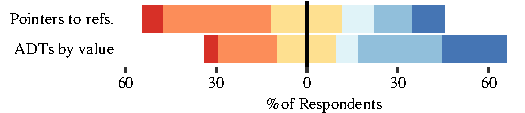
\includegraphics[width=\columnwidth]{figures/compiled/rq4_frequency_unsure.pdf}
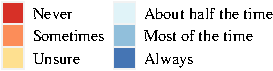
\includegraphics{figures/compiled/legends/legend_frequency_unsure_wrapped.pdf}
\end{figure}


The majority of interview participants and \ArrayItemRounded{*.feature.calling.foreign.functions}\% of survey respondents used Rust's foreign function interface (FFI). Multiple prior studies of Rust developers~\cite{holtervennhoff23,fulton21,astrauskas20} have also found that FFI use is common. Most participants found it difficult to reconcile the differences between Rust's memory model and foreign memory models. Participants reviewed the documentation and code from foreign libraries to ensure they were used safely, and they attempted to keep interoperation as straightforward as possible.

\FPeval{\createdbindings}{round(\ArrayItem{rq4.binding.method.i.generate.bindings.using.a.tool} + \ArrayItem{rq4.binding.method.i.write.bindings.manually} + \ArrayItem{rq4.binding.method.i.write.bindings.manually.and.generate.bindings.using.a.tool}
, 0)}

\subsubsection{Differing memory models}
Interview participants encountered several key differences between Rust and both C and C++ that made interoperation difficult. In C and C++, types can implement methods with varying thread-safety properties, but Rust's \code{Send} and \code{Sync} traits impose requirements on every behavior of a type. This made it difficult for one participant to encapsulate foreign types as wholly \code{Send} or \code{Sync} in Rust. They also noted that foreign libraries may have aliasing patterns that are fundamentally at odds with the borrow checker's restrictions. They observed that certain C APIs that receive source and destination pointers assume that the source and destination can alias, but aliasing and mutation are exclusive in Rust, so this pattern was difficult to encapsulate. Participants also noted that C allows unrestricted integer-to-pointer conversion, which is limited under Rust's strict provenance model, and that Rust's \code{Drop} semantics are different from a C++ destructor. 

To manage these differences, participants reviewed the documentation and implementation of foreign libraries to determine their safety requirements. The reverse of this situation occurred when participants exposed Rust libraries to languages with fewer safety guarantees. Implicit properties from Rust became documentation in other languages. 
\begin{pquote}{13}
...in Rust, you can trivially say, I'm going to return to you a thing, which just borrows my memory, and then you just can't access me while you're using that
...this is not very easily mappable into a C API, or rather you could do it, but then you have to read all this documentation...
\end{pquote}
Not all foreign APIs had were difficult to encapsulate, though. One participant observed that C APIs tend to expose pairs of initialization and cleanup functions for each type, which can be linked into the behavior of its Rust encapsulation. Others found that existing C APIs were easy to encapsulate since \ilquote{there [were] no complex lifetimes involved}{11}.

\subsubsection{Simple FFI} Participants attempted to keep interoperation with foreign code as straightforward as possible. When declaring bindings, one participant preferred  using primitive types and pointers over abstract data types like \code{Option} and \code{NonNull}, even though these types can be implicitly cast into raw pointers. They felt that these casts hid useful contextual information, so they preferred to use raw pointers explicitly.

\FPeval{\avoidedadts}{round(\ArrayItem{rq4.adts.avoided.always} + \ArrayItem{rq4.adts.avoided.most.of.the.time},0)}

A few participants indicated that they would avoid passing structs by value in certain situations. One of these participants found that certain Rust programs would behave incorrectly when structs were moved across a foreign boundary instead of copied, or if they had a destructor on the \CC{} side of the boundary. They typically avoided passing structs by value in either situation, and they recommended that \ilquote{...if you're doing FFI, the only things you should pass by value are \code{Copy} types}{2}. In most cases, participants felt comfortable passing structs by value if they were \code{Copy} and had equivalent layouts on each side of the boundary. However, as shown in Figure~\ref{fig:rq4:types}, nearly half (\avoidedadts\%) of survey respondents avoided passing abstract data types at least half of the time, if not more, suggesting that this practice is not universally followed.
 
In addition to limiting the use of certain types at boundaries, interview participants also attempted to minimize the interactions between each side of the FFI boundary. They thought that a \ilquote{very chatty API}{7} would be difficult to validate. One participant described the complexity of a foreign API in terms of the heap object graph that is exposed to Rust. They perceived that if the structure of the foreign heap is exposed in detail, then it will make safe encapsulations difficult to use.

\begin{pquote}{14}
It's hard to keep those objects around for very long unless you want all of your structs to end up with a bunch of lifetimes...
you don't want that...
it'll scare away new programmers for sure.
\end{pquote}
\FPeval{\avoidedrawasref}{round(\ArrayItem{rq4.raw.asref.avoided.most.of.the.time} + \ArrayItem{rq4.raw.asref.avoided.always},0)}
Survey respondents found it difficult to avoid converting foreign raw pointers into Rust's reference types; only \avoidedrawasref\% actively avoided this more than half of the time, as shown in Figure~\ref{fig:rq4:types}. This does not necessarily indicate that foreign heap objects tend to span FFI boundaries, but it does suggest that invalid pointer-to-reference casts may be a significant, unchecked source of undefined behavior, since Rust-specific development tools have limited support for foreign function calls. 

\rsqfour 
Developers perceived that certain API patterns were easy to encapsulate. However, unlike Holtervennhoff et al.~\cite{holtervennhoff23}, interview participants typically found it difficult to use foreign functions correctly because their aliasing and thread-safety properties were opaque and conflicted with the restrictions of the borrow checker and other Rust idioms. Participants minimized their interaction with foreign code to mitigate these differences. Some interview participants and survey respondents avoided passing structs by value, but survey respondents were not likely to avoid converting foreign raw pointers into safe references. 